\section{DME Overview}
\label{sec:dme-overview}

\subsection{Task Formulation and Retrieval Setting}
\label{sec:task-formulation}

DME is designed for instruction-aware universal multimodal retrieval. We use the term ``document'' to denote a generic retrievable item, which may be a text passage, an image, a video or a mixed-modality object. Similarly, a query may also be text-only, vision-only, video-based, or composed of multiple modalities. This setting covers a broad family of retrieval tasks, including text-to-text retrieval, text-to-image retrieval, image-to-text retrieval, video retrieval, visual document retrieval, multimodal question answering, classification-as-retrieval, and moment-level retrieval~\cite{MMEB,VLM2VecV2,Qwen3VLEmbedding,ColPali,visrag}.

Formally, let $\mathcal{X}$ denote the space of multimodal instances. Each instance $x \in \mathcal{X}$ is represented as a token sequence constructed from one or more modalities:
\begin{equation}
    x = [x^{\mathrm{text}}, x^{\mathrm{image}}, x^{\mathrm{video}}],
\end{equation}
where absent modalities are omitted. A retrieval task is specified by a natural-language instruction $\iota$, which defines the relevance criterion between a query and a document. For example, the instruction may ask the model to retrieve an image matching a textual description, find a document that answers a question, classify an input by retrieving the correct label, or locate a video segment corresponding to a temporal event.

We organize training and evaluation data as a collection of task-specific retrieval datasets:
\begin{equation}
    \mathcal{D} = \{\mathcal{D}_m\}_{m=1}^{M},
    \qquad
    \mathcal{D}_m = (\iota_m, \mathcal{Q}_m, \mathcal{C}_m, \mathcal{R}_m),
\end{equation}
where $\iota_m$ is the task instruction, $\mathcal{Q}_m$ is the query set, $\mathcal{C}_m$ is the candidate corpus, and $\mathcal{R}_m$ contains relevance annotations. For each query $q_i \in \mathcal{Q}_m$, the relevance annotation is written as
\begin{equation}
    \mathcal{R}_m(q_i) = (\mathcal{P}_i, \mathcal{N}_i),
\end{equation}
where $\mathcal{P}_i \subset \mathcal{C}_m$ denotes relevant documents and $\mathcal{N}_i \subset \mathcal{C}_m$ denotes irrelevant or hard-negative documents. The learning objective is to produce a scoring function that ranks documents in $\mathcal{P}_i$ above those in $\mathcal{N}_i$:
\begin{equation}
    s_\theta(q_i, d^+ \mid \iota_m) > s_\theta(q_i, d^- \mid \iota_m),
    \quad
    d^+ \in \mathcal{P}_i,\ d^- \in \mathcal{N}_i.
\end{equation}

DME follows a bi-encoder retrieval setting. Given an instruction $\iota$, a query $q$, and a document $d$, the model independently encodes the query and document into dense vectors:
\begin{equation}
    \mathbf{z}_q
    =
    E_{\theta}^{q}
    \left(
        T_q(\iota,q)
    \right),
    \qquad
    \mathbf{z}_d
    =
    E_{\theta}^{d}
    \left(
        T_d(\iota,d)
    \right),
\label{eq:bi-encoder-extraction}
\end{equation}
where $T_q$ and $T_d$ are query-side and document-side input templates, and $E_{\theta}^{q}$ and $E_{\theta}^{d}$ denote the corresponding embedding extraction procedures. Both extractors share the same MLLM backbone and embedding projection, while allowing side-specific retrieval-token layouts and readout functions. The resulting embeddings are $\ell_2$-normalized.

The relevance score is computed by inner product, which is equivalent to cosine similarity after normalization:
\begin{equation}
    s_\theta(q,d\mid\iota)
    =
    \mathbf{z}_q^\top \mathbf{z}_d.
\label{eq:retrieval-score}
\end{equation}

At inference time, all document embeddings in the corpus are computed offline and stored in an approximate nearest-neighbor index. Given an online query, DME performs a single query-side encoding pass and retrieves candidates by vector similarity:
\begin{equation}
    \operatorname{Retrieve}(q, \mathcal{C})
    =
    \operatorname{TopK}_{d \in \mathcal{C}}
    \ s_\theta(q, d \mid \iota).
\end{equation}
This retrieval setting is critical for large-scale deployment because it avoids pairwise cross-attention between the query and every candidate document. It also separates training-time supervision from inference-time computation.

% Although DME maps both sides into a shared embedding space and uses a symmetric vector similarity function, the retrieval formulation remains role-conditioned. Queries and documents play different semantic roles: the query defines the retrieval intent and relevance criterion, while the document provides candidate evidence or target content. This role-conditioned asymmetry is implemented through query-side and document-side input templates. It is also useful for the Stage-2 cross-conditional objectives, where query representations are encouraged to preserve document-side semantics and document representations are encouraged to preserve query-side semantics.

\subsection{Model Architecture and Embedding Extraction}
\label{sec:model-architecture-embedding}

DME is built on a generative multimodal large language model as a shared embedding backbone. The backbone receives an instruction-aware serialized sequence consisting of text tokens, visual tokens, and retrieval-specific tokens. The visual tokens may come from images, video frames, visual documents, or other visual inputs. Following recent MLLM-based embedding models~\cite{E5-V,GME,MMEB,VLM2VecV2,Qwen3VLEmbedding}, DME converts the generative backbone into a dense retriever by extracting compact vector representations from retrieval-side hidden states.

Given a retrieval instruction $\iota$ and a multimodal instance $x$, DME constructs the input sequence as:
\begin{equation}
    \mathbf{u}
    =
    T(\iota, x)
    =
    [
    \mathbf{u}_{\mathrm{inst}};
    \mathbf{u}_{x};
    \mathbf{u}_{\mathrm{ret}}
    ],
\end{equation}
where $\mathbf{u}_{\mathrm{inst}}$ denotes the instruction tokens, $\mathbf{u}_{x}$ denotes the serialized multimodal content, and $\mathbf{u}_{\mathrm{ret}}$ denotes retrieval-specific tokens appended after the input content. Since these retrieval tokens are placed at the end of the sequence, their hidden states can attend to the preceding multimodal context under the causal attention mechanism of the MLLM backbone.

Let $F_{\theta}$ denote the MLLM backbone. Given the serialized sequence $\mathbf{u}$, the model produces final-layer hidden states:
\begin{equation}
    \mathbf{H}
    =
    F_{\theta}(\mathbf{u})
    =
    [
    \mathbf{h}_1,
    \mathbf{h}_2,
    \ldots,
    \mathbf{h}_{|\mathbf{u}|}
    ].
\end{equation}
DME extracts a readout representation $\mathbf{r}$ from the retrieval-specific hidden states and projects it into the embedding space:
\begin{equation}
    \mathbf{z}
    =
    \operatorname{norm}
    \left(
        W_{\mathrm{emb}}
        \mathbf{r}
    \right),
\end{equation}
where $W_{\mathrm{emb}}$ is the embedding projection matrix and $\operatorname{norm}(\cdot)$ denotes $\ell_2$ normalization. The concrete construction of $\mathbf{r}$ differs across training stages and is summarized in Section~\ref{sec:two-stage-learning-pipeline}.

The side-specific extraction functions $E_{\theta}^{q}$ and $E_{\theta}^{d}$ are defined in Eq.~\eqref{eq:bi-encoder-extraction}. They share the same MLLM backbone and embedding projection, but may use different retrieval-token layouts and readout functions. In Stage 2, both query and document inputs may use modality-aware anchor tokens for evidence grounding, while typed latent reasoning is introduced on the query side. The resulting normalized embeddings are compared using the score in Eq.~\eqref{eq:retrieval-score}.

\subsection{Two-Stage Learning Pipeline}
\label{sec:two-stage-learning-pipeline}

% \begin{figure*}[tp]
%     \centering
%     \includegraphics[width=\linewidth]{images/fig2_pipeline.pdf}
%     % \vspace{-18pt}
% \caption{\textbf{Overview of the PDF-VLM2Vec Pipeline.} 

\begin{figure*}[tp]
    \centering
    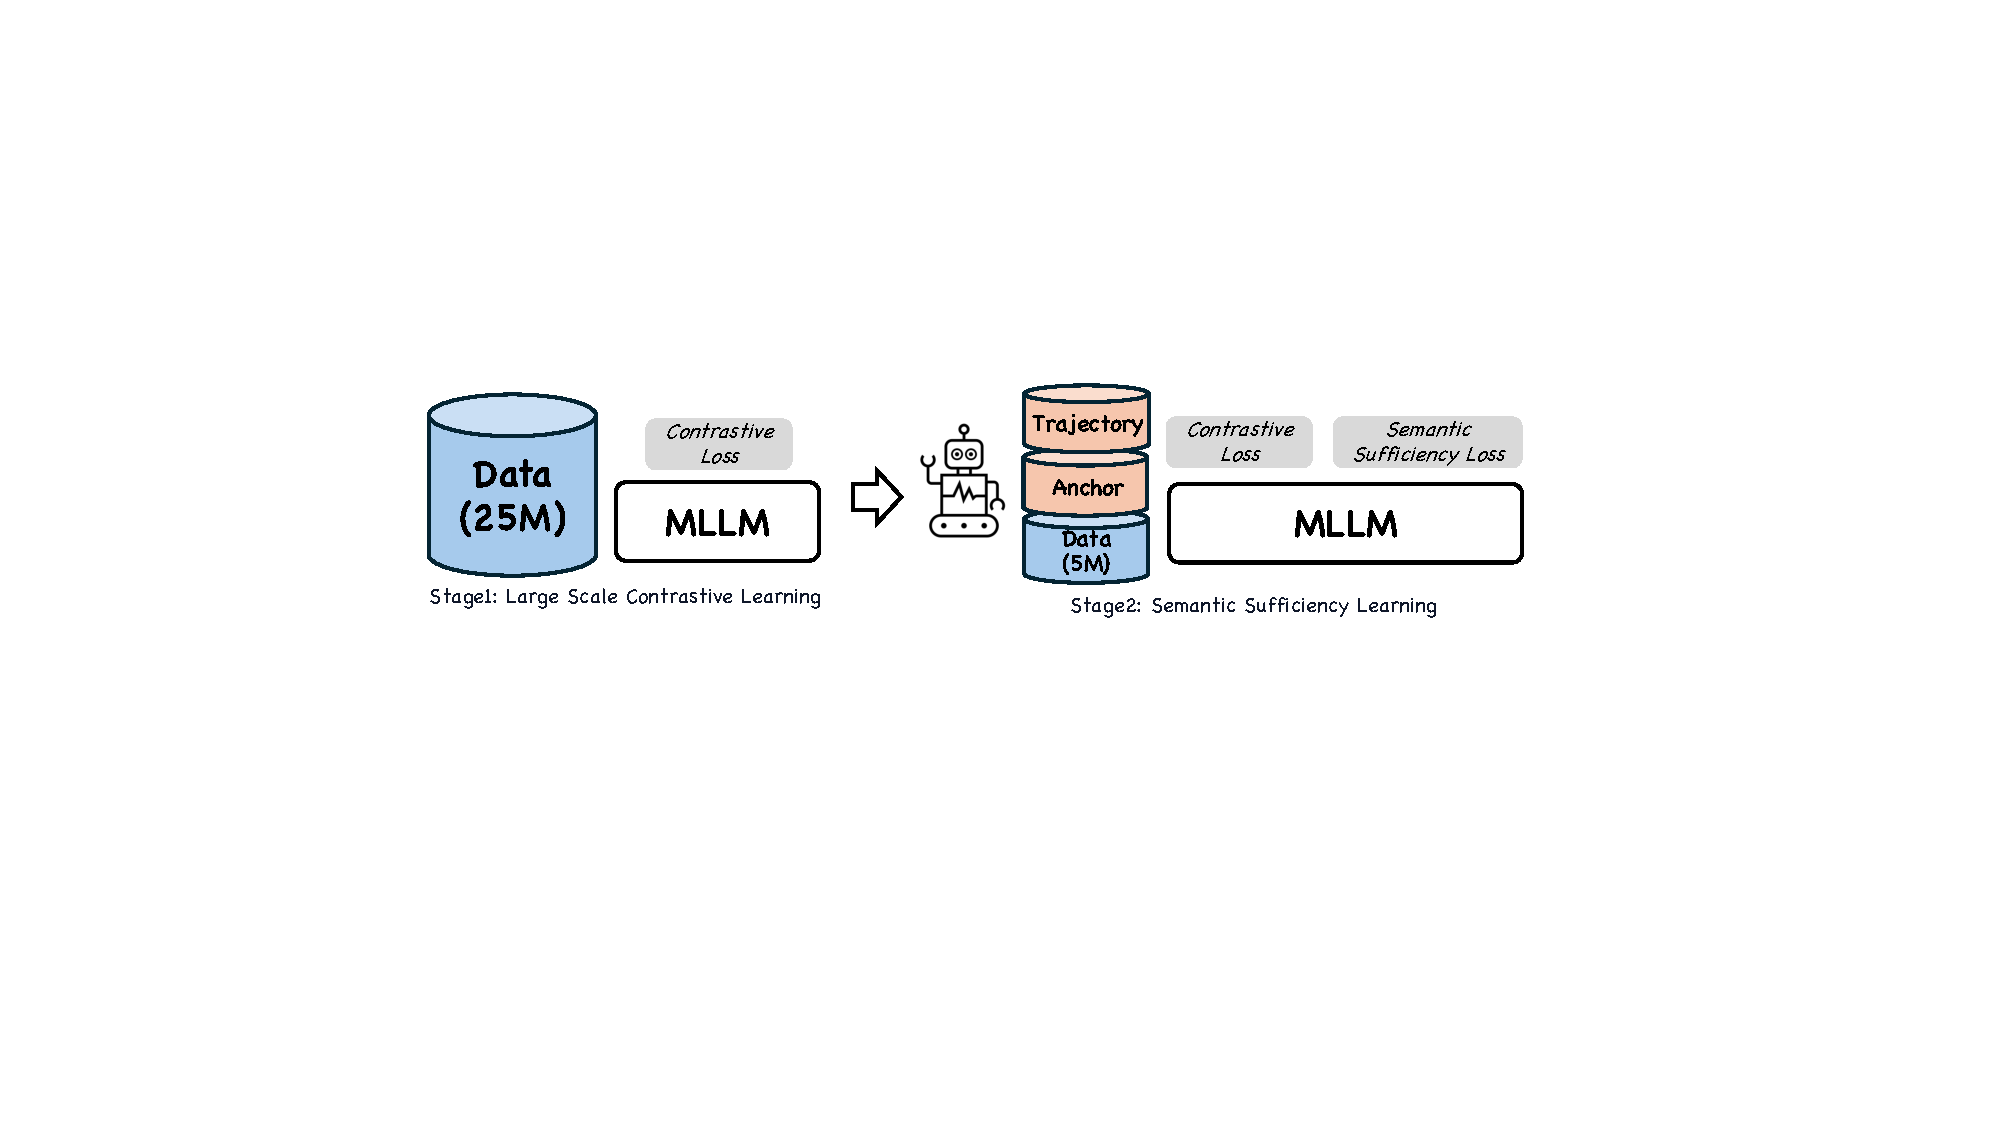
\includegraphics[width=1\linewidth]{figures/fig-pipeline.pdf}
    \caption{\textbf{Overview of the DME two-stage training pipeline.}
    In Stage 1, the MLLM backbone is
    trained on 25M multimodal query-target pairs with a contrastive loss to
    establish a scalable bi-encoder embedding space.
    In Stage 2, the model is further
    refined on a smaller, higher-quality set of 5M examples augmented with
    teacher-generated CoT supervision. Stage 2 is optimized
    jointly by the contrastive loss and a semantic sufficiency loss, the latter
    combining Evidence-Grounded Typed Latent Reasoning and Cross-Conditional
    Reconstruction. Cross-Conditional Reconstruction is used only during training. The latent tokens remain inside a single-pass encoder and introduce only marginal query-side overhead, while retrieval is still performed through standard dense-vector similarity.}
    \label{fig:pipeline}
  \label{fig:pipeline}
\end{figure*}

DME is trained in two major stages, as shown in Figure~\ref{fig:pipeline}. Stage 1 builds a broad multimodal embedding space through large-scale contrastive pre-training, while Stage 2 improves the semantic sufficiency of the learned representations through evidence-grounded latent reasoning and cross-conditional reconstruction. The detailed objectives are introduced in Section~\ref{sec:multi-stage-learning-framework}; here we summarize the overall pipeline and how each stage changes the retrieval readout.

\textbf{Stage 1: large-scale contrastive pre-training.}
In the first stage, DME uses a standard embedding token as the retrieval-specific token:
\begin{equation}
    \mathbf{u}_{\mathrm{ret}}^{(1)}
    =
    [
    \texttt{<emb>}
    ].
\end{equation}
The readout representation is obtained from the final hidden state of this token:
\begin{equation}
    \mathbf{r}^{(1)}
    =
    \mathbf{h}_{\texttt{<emb>}},
    \qquad
    \mathbf{z}^{(1)}
    =
    \operatorname{norm}
    \left(
        W_{\mathrm{emb}}
        \mathbf{r}^{(1)}
    \right).
\end{equation}
This simple readout allows DME to scale contrastive pre-training over heterogeneous query--document pairs, including text, image, video, visual document, and mixed-modality data. The goal of this stage is to establish broad modality alignment and a stable initial retrieval geometry.

\begin{figure*}[t]
    \centering
    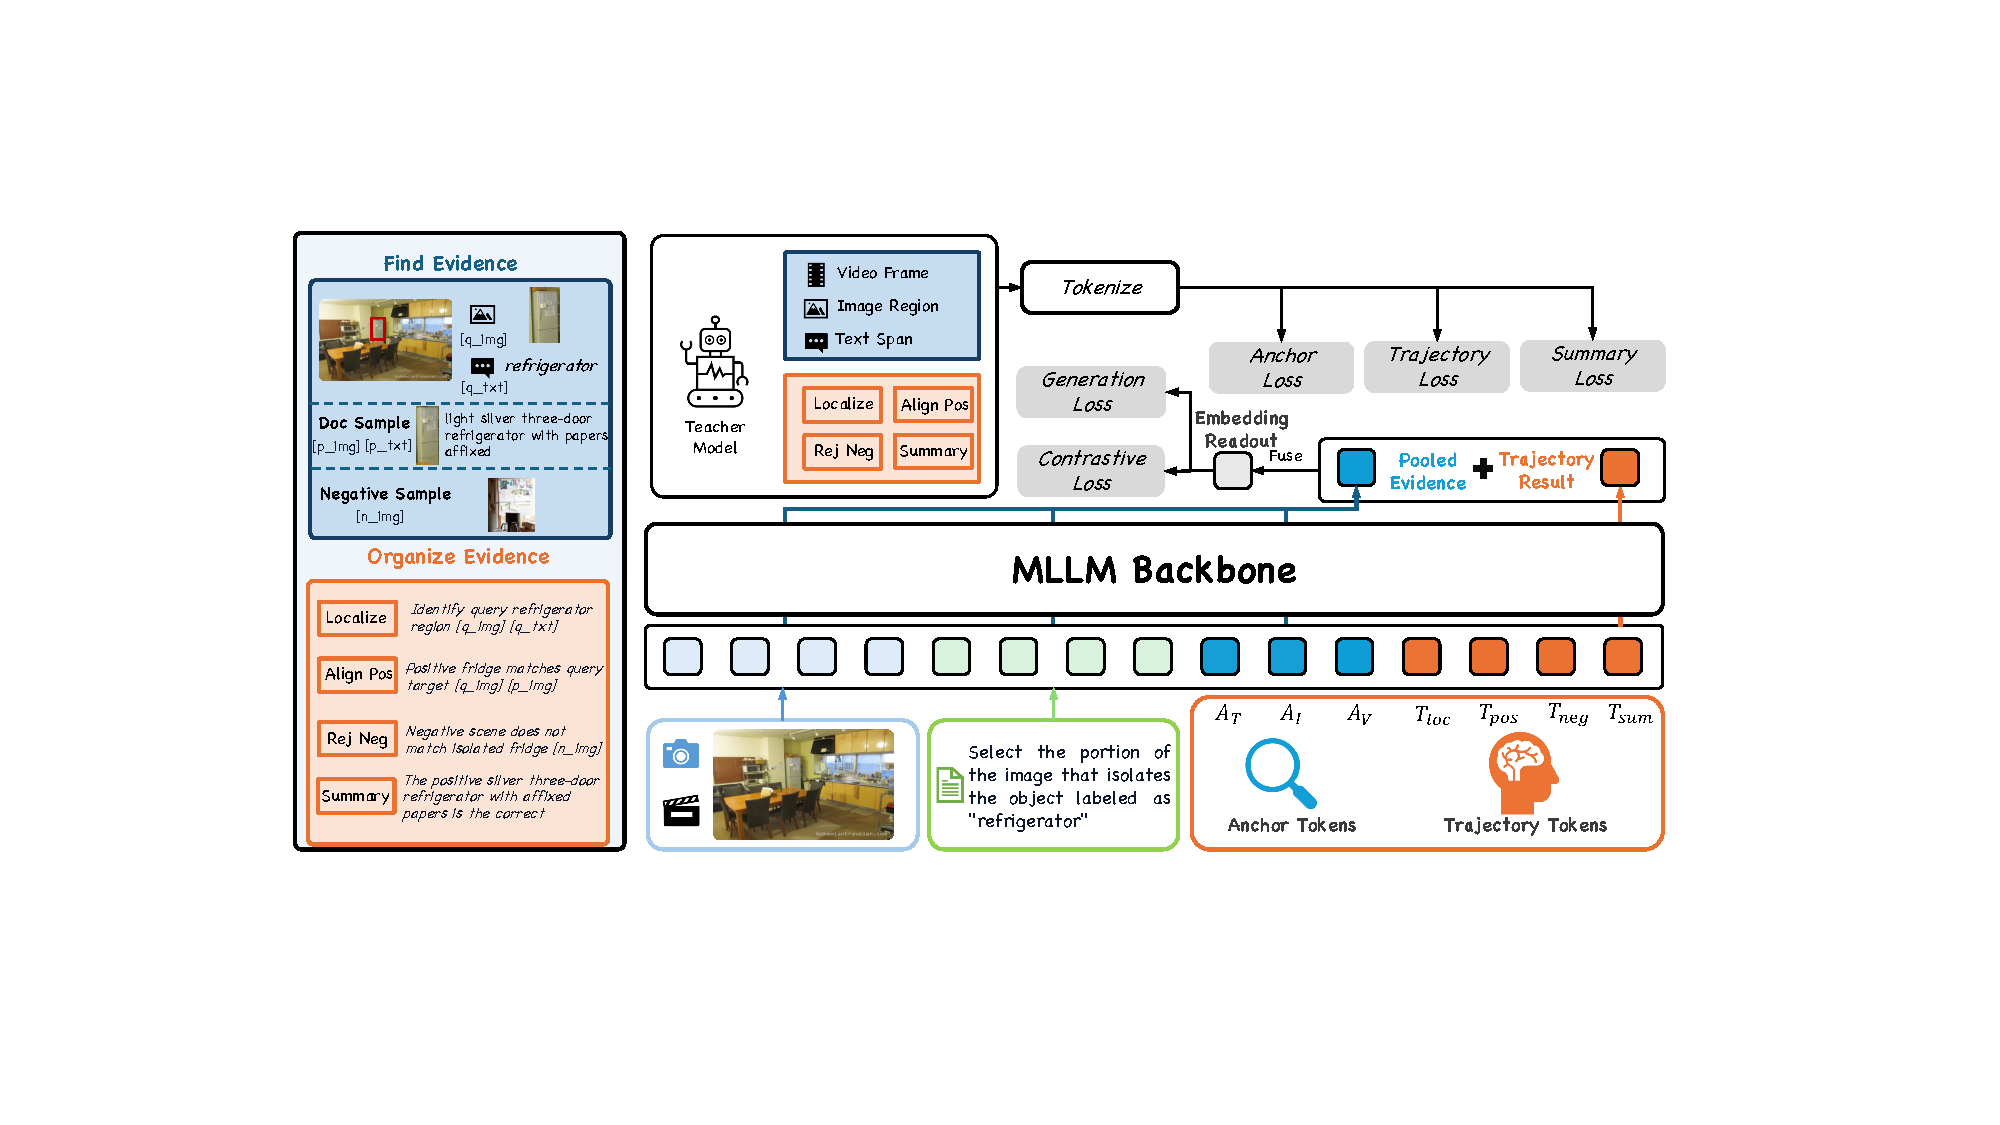
\includegraphics[width=1\linewidth]{figures/fig-pipeline-stage2.pdf}
\caption{\textbf{Stage 2: Semantic Sufficiency Learning.}
A teacher model decomposes a query--positive--negative triplet into localized multimodal evidence and typed retrieval states. These signals supervise modality-aware anchor tokens and query-side latent states, whose terminal state is combined with pooled evidence to form the retrieval representation. Cross-Conditional Reconstruction provides an additional NTP/MTP objective during training, shown as the generation loss in the figure. At evaluation time, DME performs a single encoder forward pass without explicit textual CoT generation or reconstruction.}
\label{fig:stage2}
\end{figure*}

\textbf{Stage 2: semantic sufficiency learning.}
Stage 2 retains the same normalized embedding interface while introducing two complementary mechanisms (Figure~\ref{fig:stage2}). Both query and document inputs may use modality-aware anchor tokens for evidence grounding. The query side additionally uses a small number of typed latent states, whose terminal state contributes to the query readout, while the document side retains a standard document readout. Stage 2-A uses these representations for Evidence-Grounded Typed Latent Reasoning, and Stage 2-B further uses the readout representations as conditioning prefixes for NTP/MTP-based reconstruction during training. The detailed formulations are provided in Sections~\ref{sec:stage2a-typed-latent-reasoning} and~\ref{sec:stage2b-cross-conditional-self-decoding}.


